\documentclass[11pt]{article}

% set these commands
\newcommand{\course}{CSCI 534}
\newcommand{\proj}{Homework 03}
\newcommand{\dueDate}{3-9-2021}
\newcommand{\instructor}{David L. Millman}

\usepackage{../macros}

\begin{document}

\coverpage{03}

\newpage
\section*{Problem 1}

Given an polygonal chain $P$ of $n$ vertices, we define an vertex $v$ as a
\emph{local max} if $v$ if all edges adjacent to $v$ are to the left of $v$.
Show that can determine if a polygonal chain with $k$ local maxes is simple in
$O(n \log k)$ time. \\\\
\answer

\newpage
\section*{Problem 2}

A friend of yours from the civil engineering department wants to analyze whether
a dangerous portion of a river will flood. He presents you with the following
(admittedly rather unrealistic) model of the river. The portion of the river of
interest is modeled as an $x$-monotone polygon $P$ that is bounded between two
vertical lines at $x = x^-$ and $x = x^+$ (see Figure). The river is bounded on
its left and right ends by two vertical line segments of lengths $w^-$ and
$w^+$, respectively. Inside the polygon are some number of disjoint x-monotone
polygons that represent islands in the river.  Let $n$ denote the total number
of vertices, including both the outer banks of the river and the islands.

\begin{figure}[h]
    \centering
    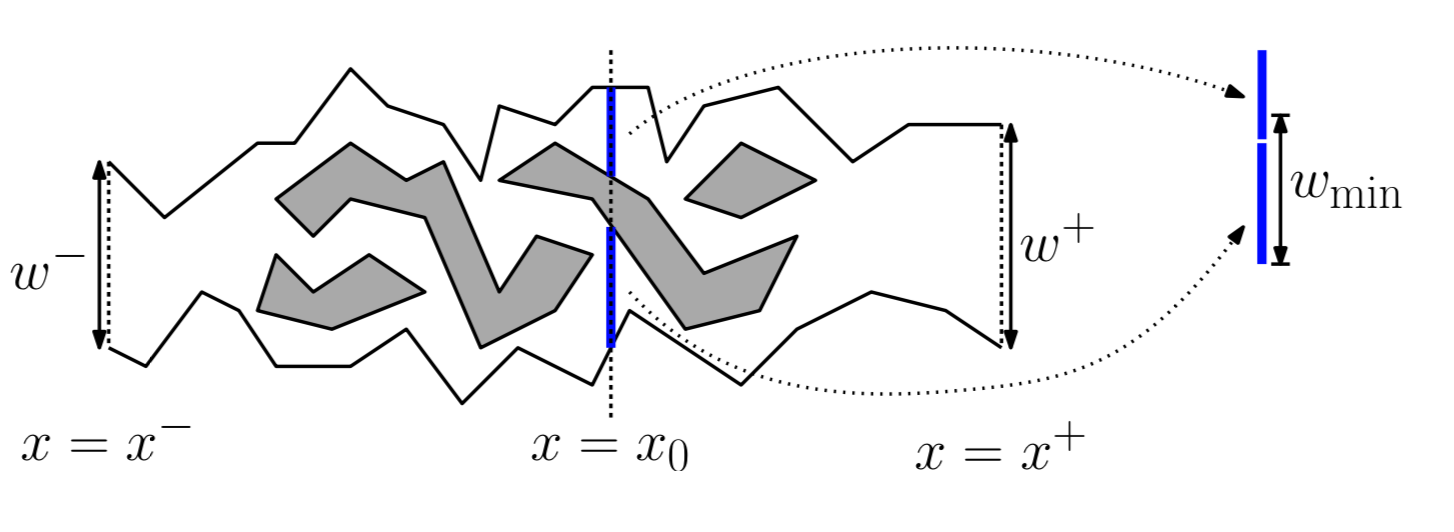
\includegraphics[width=0.75\textwidth]{river}
    \caption{Problem 2: River}
\end{figure}

Your friend tells you that in order to avoid a flood, the width of the river
(not counting islands) at every vertical cut must be at least some minimum value
$w_{min}$. For example, in the figure, the sum of the two blue vertical segments
at $x = x_0$ must be at least $w_{min}$ in order to avoid a flood.  Given the
polygon $P$ and the value $w_{min}$, present an $O(n \log n)$ time algorithm that
determines whether the river will flood, that is, whether there is a vertical
cut whose total width is smaller than $w_{min}$. If it will flood, your algorithm
should output the value $x_0$ of the bottleneck, that is, the location where the
sum of vertical lengths (excluding islands) is the smallest. \\\\
\answer
This problem ended up have a very clean solution which we liked a lot!
We settled on a sweep line algorithm.
We got our inspiration from the original sweep line algorithm that we learned about: line segement intersection.
Although all we care about is whether a polygon (island) is on the sweep line or not, so we can ignore its neighbors.
This means we do not have to maintain an ordered dictionary as our sweep line data structure, instead we can use an array with constant time access!

Before giving a description of the algorithm, let's discuss some assumptions.
First, assume that each polygon is stored in an array with the vertices ordered counter clockwise.
As far as general position goes, we assume that no two vertices have the same $x$-coordinate (with the exception of the left and right points of the river).
The event points will be vertices so this means all events will have different $x$-coordinates.

Now we describe the algorithm.
For input, our algorithm will take in the array representing the shore $S$ and the arrays representing each island $I_i$ together with the values $w^-$, $w^+$, and $w_{min}$.
As noted before, the vertices become the event points.
We have two types of event points: one that contains a vertex of $S$ and another which contains a vertex of some $I_i$.
So we sort the events according to their $x$-coordinates and store the result in a queue.
There will not be any more event points so a regular queue will suffice.
Now we will compute the river width each event point (we will provide a proof that considering the vertices is sufficient).

One way to compute the width at $x^\star$ is to subtract the width of each island on the sweep line at $x^\star$ from the distance between the shoreline $S$.
The problem with this is that we can construct input with $\Omega (n)$ islands at some $x^\star$.
One such input is a approximately $n/3$ triangles stacked vertically.
This would result in an $O(n^2)$ algorithm.

To bypass this, note that the width of the river at any point can be modeled as a piecewise-linear continuous function.
All we have to do is find the appropriate line segments and perform $O(1)$ operations at each event point.
With this model, we can reduce what we store on the sweep line.
All we need is the function representing the current line segment.
We don't even need to store what islands the sweep line is intersecting because we can determine the event type just by inspecting which polygon a point comes from!

Now let's figure out the a function for the first line segment.
We assumed no two event points have the same $x$-coordinate, so there exists some interval $A$ for which the left side of the river matches Figure \ref{fig:basecase}.
Figure $\ref{fig:basecase}$ also depicts the function representing the first line segment.
The top line has slope $s_1$ and the bottom line has slope $s_2$.
Certainly we begin with width $w^-$ and then for any $x$ beyond $x_0$ we can add $s_1 x$ and subtract $s_2 x$ to obtain the width at $x$.
The function $w_A (x)$ accurately reports the width on the inteval $[x_0, x^\star]$ where $x^\star$ is the $x$-coordinate of the next event point.

\begin{figure}[h]
    \centering
    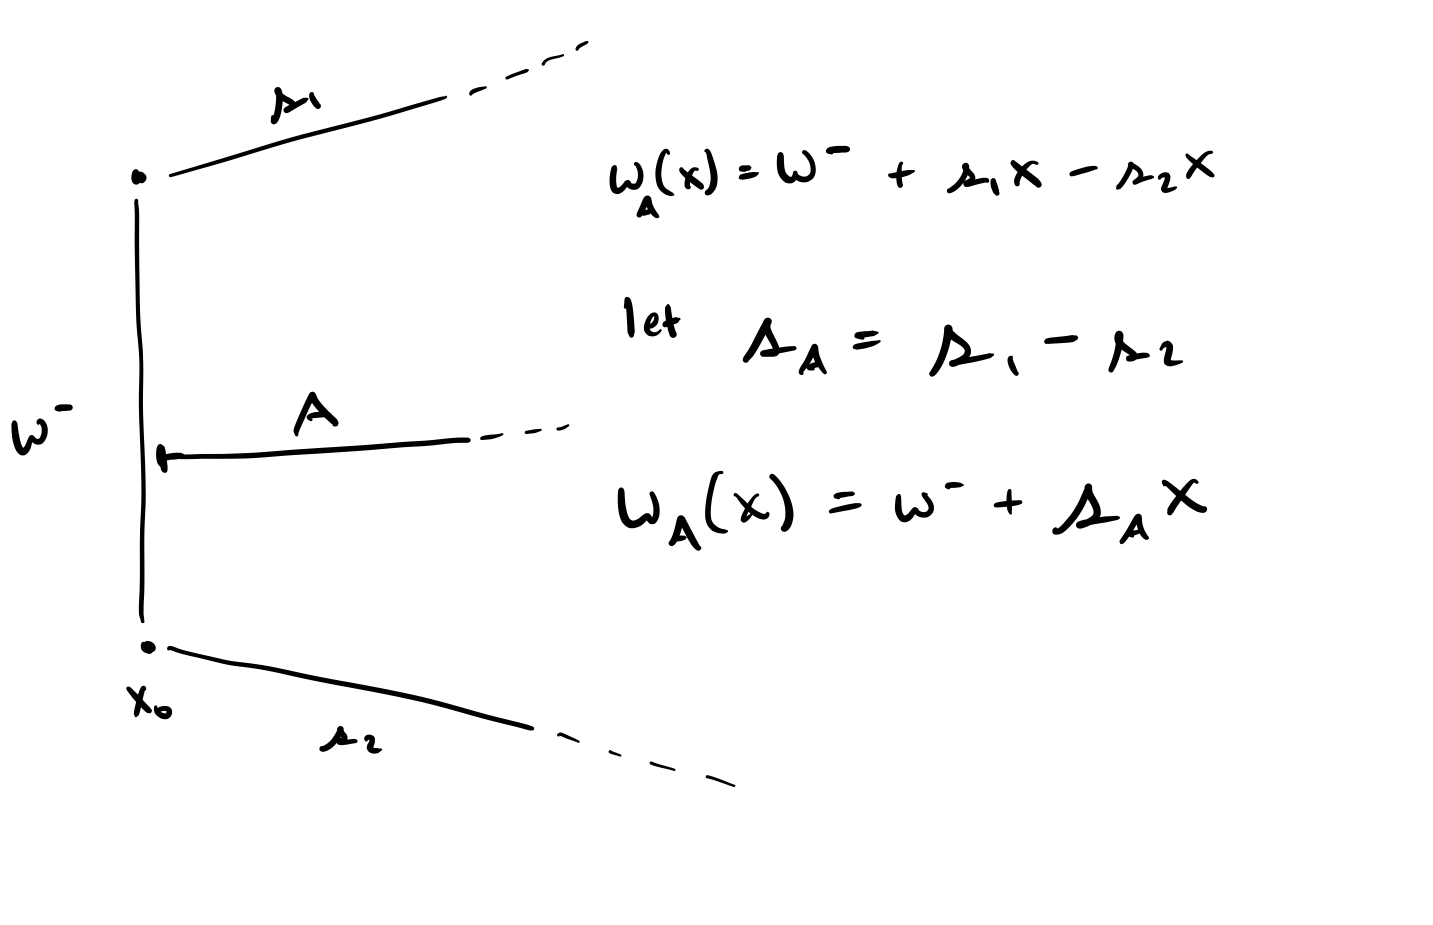
\includegraphics[width=0.6\textwidth]{basecase}
    \caption{Base case depiction}
    \label{fig:basecase}
\end{figure}

At $x^\star$, the $x$-coordinate of the next event point, we can enter one of four cases.
In case 1, the event contains a vertex from $S$ the shore line.
Case 1 in Figure \ref{fig:updateswp} depicts how $w_A(x)$ transforms into $w_B(x)$ if the vertex is part of the upper shoreline.
An analagous operation occurs for the lower shoreline.
The remaining 3 cases show what happens if the even contains a vertex from an island $I_i$.
We can determine which case to enter by inspecting the neigboring points of the vertex in $I_i$.
Case 2 covers what to do when an island begins and Case 4 shows what happens when an island ends.
Case 3 depicts how $w_B (x)$ is constructed when the vertex is on the upper part of an island and there is analogous operation when the vertex is on the lower part of an island.

\begin{figure}[h]
    \centering
    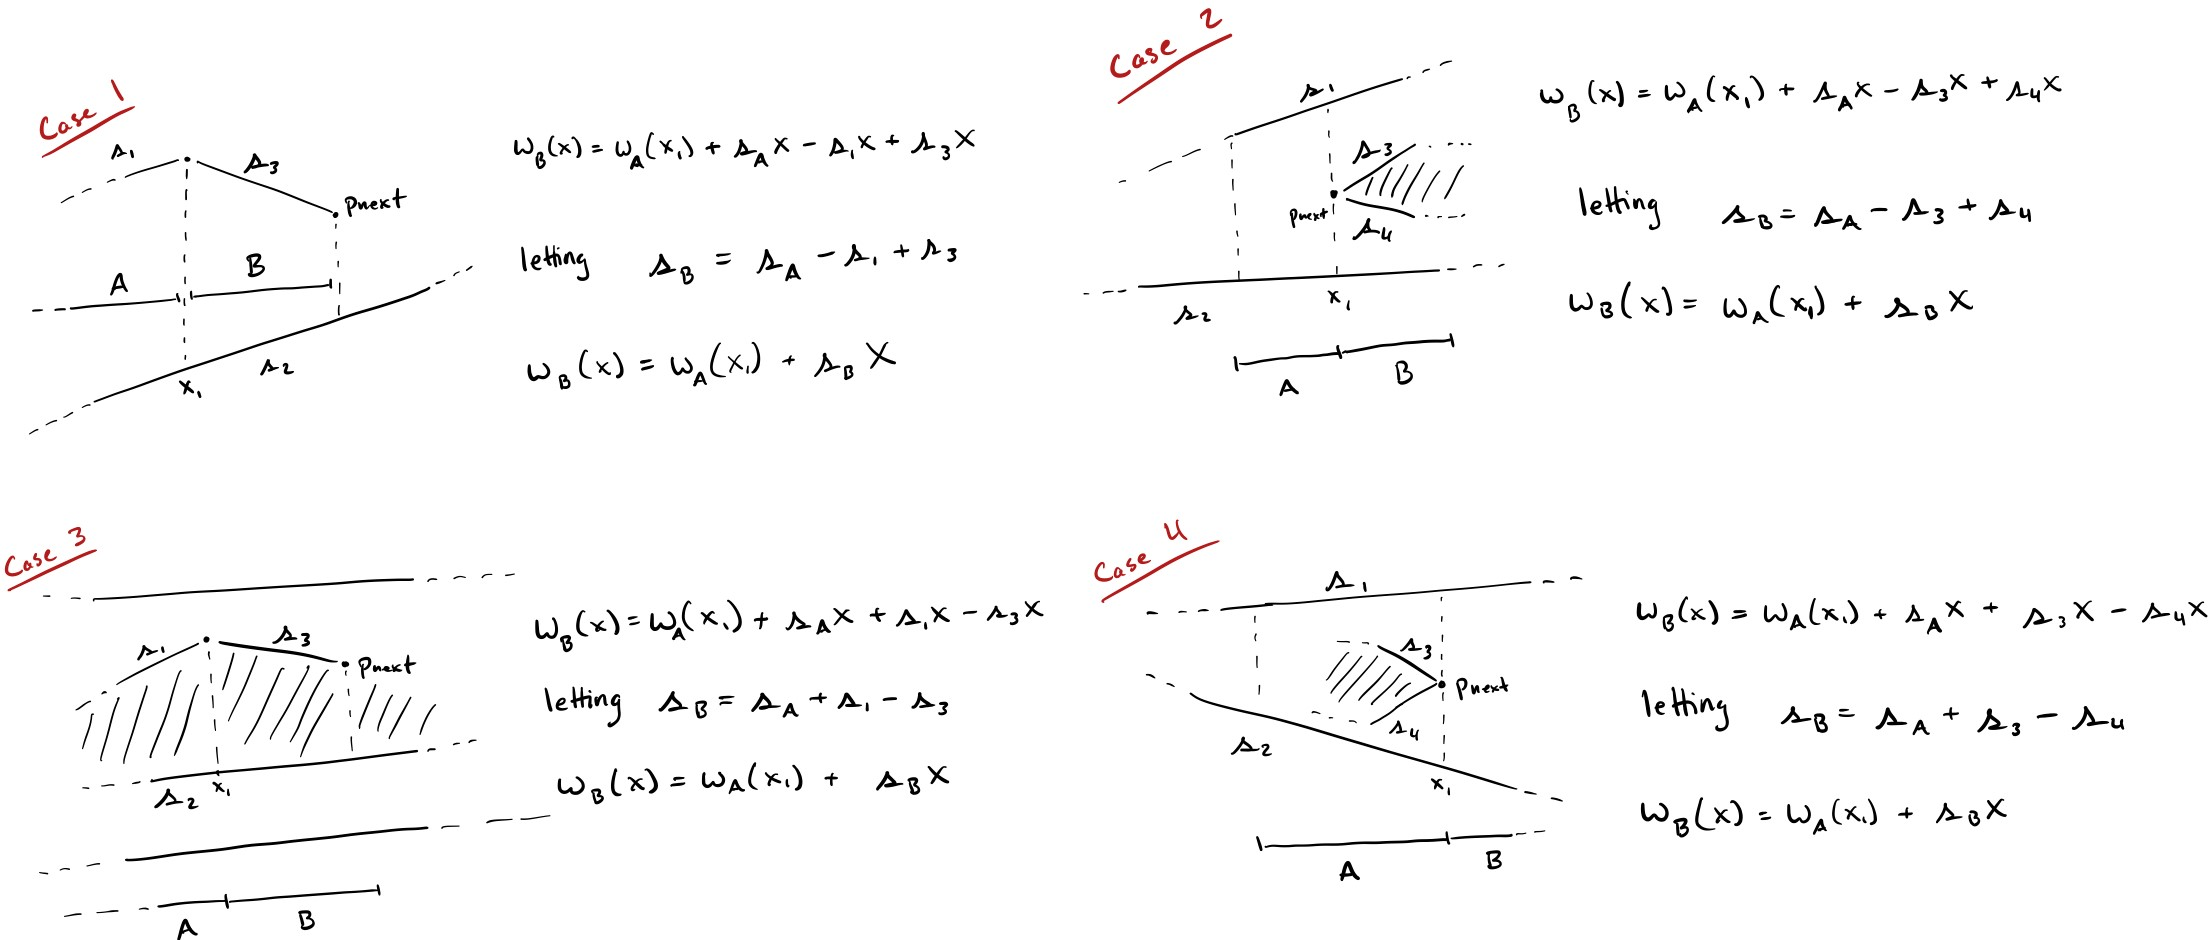
\includegraphics[width=\textwidth]{updateswp}
    \caption{Cases for updating the sweep line}
    \label{fig:updateswp}
\end{figure}

As we consider each event point, we can keep track of the smallest width found so far and the $x$-coordinate that is occurs at.
In keeping with our piecewise-linear continuous model for the width of the river let's store them in variables called $min_x$ for the $x$-coordinate and $min_y$ for the width of the river at $min_x$.
When the sweep terminates, if $min_y < w_{min}$ return $min_x$, otherwise return NO FLOOD.

Before discussing correctness, let's look at run time.
There are two bigs steps in this algorithm.
The first is sorting $n$ points which takes $O(n \log n)$ time.
The next big step is to process the $n$ events.
In every case, we perform a constant number of operations so the run time for this step is $n * O(1) = O(n)$.
Therefore the entire run time is $O(n \log n) + O(n) = O(n \log n)$ as desired.

TODO: prove correctness

\newpage
\section*{Problem 3}

\begin{enumerate}

    \item (7 points) Describe and analyze an algorithm that computes the
        convex hull of a set of $n$ points in the plane using randomized
        incremental construction in expected $O(n \log n)$ time. For this
        problem you are welcome to find an algorithm and its analysis on the
        web, but please cite where you found it, describe it concisely in
        your own words, and make the analysis very concise. Where does the
        log-factor come from?

    \item (3 points) Give an example of a set of points in the plane, and a
        particular input order, that causes the convex hull algorithm to run in
        $O(n^2)$ when the points are added in this particular order. Make sure it
        is clear how your example generalizes to arbitrary values of $n$.

\end{enumerate}
\answer

\newpage
\section*{Problem 4}

Consider the following instance of the trapezoidal map point location data
structure. The left side shows the map, and the right side shows the
corresponding DAG. Describe the resulting trapezoidal map and DAG after segment
$xy$ has been added.

\begin{figure}[h]
    \centering
    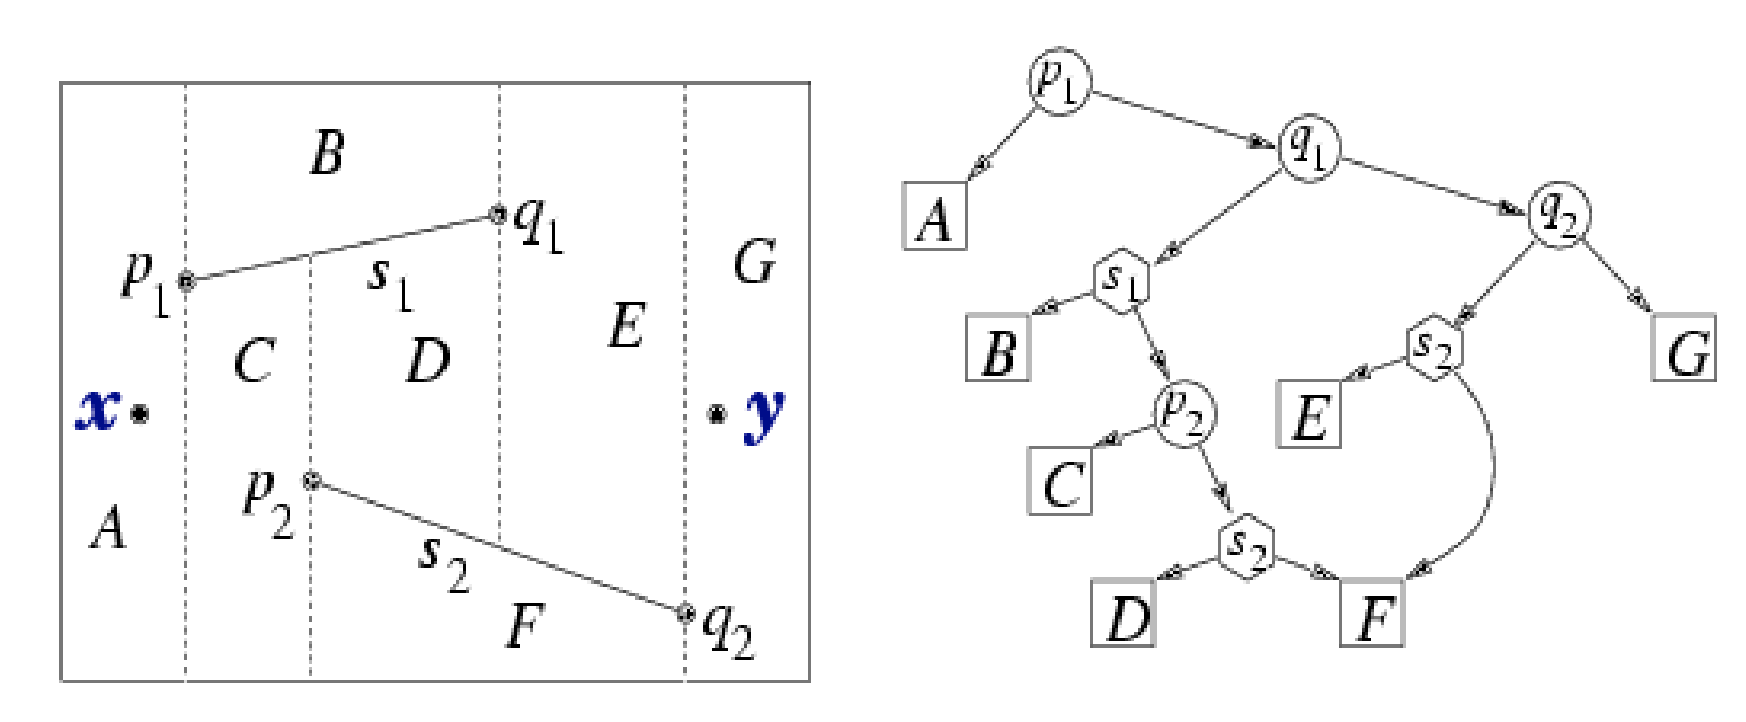
\includegraphics[width=0.75\textwidth]{trapMap}
    \caption{Problem 4: Trapezoid Map}
\end{figure}
\answer

\newpage
\section*{Problem 5}

Consider the following algorithm:

\begin{verbatim}
    FindMax(A,n){
        // Finds maximum in set A of n numbers
        if(n==1) return the single number in A
        else {
            x = extract random element from A // in constant time; x is removed from
            A
            y = FindMax(A,n-1)
            if(x<=y) return y;
            else
            Compare x with all remaining elements in A and return the maximum
        }
    }
\end{verbatim}

\begin{enumerate}

\item (4 points) Argue that this algorithm is correct, and give its worst-case
    runtime. (The runtime is proportional to the number of comparisons made.)

\item (6 points) Compute the expected runtime of this algorithm.  (Hint:
    Introduce an indicator random variable for executing the else branch in the
        $i$-th step, and use backwards analysis to simplify the analysis.)

\end{enumerate}
\answer

\end{document}
